    %%!TEX root = ./UserManual.tex
\chapter{Appendices}
\label{chap:appendices}

%%%%%%%%%%%%%%%%%%%%%%%%%%%%%%%%%%%%%%%%%%%%%%%%%%%%%%%%%%%%%%%%
% Updated configuration file
%%%%%%%%%%%%%%%%%%%%%%%%%%%%%%%%%%%%%%%%%%%%%%%%%%%%%%%%%%%%%%%%
\section{Updated configuration file}
\label{section:updated_config_file}

In this section we will show you which updates were made to the configuration file, and explain what their effect will be on the simulation.\\
Below is an example of the new configuration file when generating the population with multiple regions.

\begin{lstlisting}[caption={$<$geopop\_gen$>$ configuration},captionpos=b]
<geopop_gen>
<cities_file>flanders_cities.csv</cities_file>
<major_cities_file>flanders_major_cities.csv</major_cities_file>
<commuting_file>flanders_commuting.csv</commuting_file>
<workplace_file>workplace_size_distribution.csv</workplace_file>
<workplace_performance>fast</workplace_performance>
<epi_output>true</epi_output>
<epi_output_file>data.h5</epi_output_file>
<!-- Default parameters -->
<fraction_college_commuters>0.5</fraction_college_commuters>
<fraction_workplace_commuters>0.5</fraction_workplace_commuters>
<household_file>households_flanders.json</household_file>
<major_household_file>households_flanders.json</major_household_file>
<participation_preschool>0.99</participation_preschool>
<participation_daycare>0.45</participation_daycare>
<participation_college>0.5</participation_college>
<participation_workplace>0.75</participation_workplace>
<population_size>600000</population_size>
<!-- End Default parameters -->
<regions>
	<region>
		<id>1</id>
		<fraction_college_commuters>0.5</fraction_college_commuters>
		<fraction_workplace_commuters>0.5</fraction_workplace_commuters>
		<household_file>Antwerpen.json</household_file>
		<major_household_file>Antwerpen_major.json</major_household_file>
		<participation_preschool>0.99</participation_preschool>
		<participation_daycare>0.45</participation_daycare>
		<participation_college>0.5</participation_college>
		<participation_workplace>0.75</participation_workplace>
		<population_size>141971</population_size>
	</region>
	...
</regions>
</geopop_gen>
\end{lstlisting}

As you can see, you can specify the following parameters for each region:

\begin{multicols}{2}
\begin{itemize}
    \item id
    \item population\_size
    \item fraction\_workplace\_commuters
    \item fraction\_college\_commuters
    \item participation\_preschool
    \item participation\_daycare
    \item participation\_college
    \item participation\_workplace
    \item household\_file
    \item major\_household\_file
\end{itemize}
\end{multicols}

The most important one here is the id. The id of a region will correspond to the province of a city in the cities file. If the province matches no region id, the default values will be used.

To generate the files needed for the visualization tool, the parameter "epi\_output" must be true and the parameter "epi\_output\_file can be used to specify the file and format of the output.

\section{Major cities file}
\label{section:major_cities}

Here we will show an example of a major\_cities\_file file. It is pretty self explanatory, since it is just a CSV file containing the ID's of all the cities that are defined as major.

\begin{lstlisting}[caption={major\_cities\_file example},captionpos=b]
id
11002
41002
...
\end{lstlisting}

\section{Workplace distribution file}

The workplace distribution file is a CSV file of the following form: 

\label{section:workplace_distribtion_file}

\begin{lstlisting}[caption={workplace\_file example},captionpos=b]
ratio,size_min,size_max
0.778532842256952,1,9
0.171901116625764,10,49
0.0410039025210945,50,199
0.00856213859618965,200,400
\end{lstlisting}

When specifying a workplace distribution file, it's also possible to specify a workplace performance parameter to choose between an accurate or fast implementation. The default is accurate but can be changed using:

\begin{lstlisting}[caption={workplace\_performance},captionpos=b]
<workplace_performance>fast</workplace_performance>
\end{lstlisting}

\begin{table}
\end{table}


\section{HDF5 Format} \label{hdf5_format}
\begin{figure}[!htb]
    \centering
    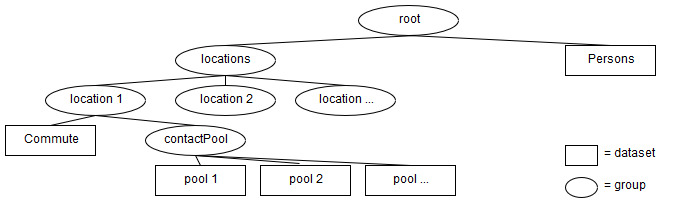
\includegraphics[width=12cm]{HDF5Format.jpg}
    \caption{Hierarchical structure}
    \label{fig:hdf5_structure}
\end{figure}

\begin{table}[!htb]
\begin{center}
\begin{tabular}{|c|c|}
\hline
to   & proportion \\ \hline
UINT & DOUBLE     \\ \hline   
\end{tabular}
\end{center}
\caption{\label{tab:commute}Dataset Commute}
\end{table}

\begin{table}[!htb]
\begin{center}
\begin{tabular}{|c|}
\hline
People    \\ \hline
UINT  \\ \hline   
\end{tabular}
\end{center}
\caption{\label{tab:pool}Dataset Pool}
\end{table}

\begin{table}[!htb]
\resizebox{\textwidth}{!}{\begin{tabular}{|c|c|c|c|c|c|c|c|c|c|}
\hline
id   & age  & k12school & household & college & workplace & primarycommunity & secondarycommunity & daycare & preschool \\ \hline
UINT & DOUBLE & UINT & UINT & UINT & UINT & UINT & UINT & UINT & UINT \\ \hline   
\end{tabular}}
\caption{\label{tab:pool}Dataset Persons}
\end{table}

A group or Dataset can contain metadata (attributes in HDF5). In Table \ref{Attributes}, the attributes of each group and dataset are shown.

\begin{table}[!htb]
\begin{center}
\begin{tabular}{|c|c|}
\hline
Dataset/Group   & Attributes \\ \hline
persons & size(rows of dataset)     \\ \hline 
locations & size(number of locations)     \\ \hline   
location x & id, name, province, population, coordinates     \\ \hline   
Commute & size(rows of dataset)     \\ \hline   
contactPools & size(number of contactPools)     \\ \hline   
People & id, type, size(rows of dataset)     \\ \hline   
\end{tabular}
\end{center}
\caption{\label{tab:commute}Attributes}
\end{table}
